\chapter{Benchmark und Modellauswahl}\label{ch:benchmark}

Die systematische Auswahl eines geeigneten \glspl{llm} erforderte die Entwicklung und Anwendung eines spezifisch auf den Anwendungsfall zugeschnittenen Benchmarks.
Die Konzeption und Durchführung war ein iterativer Prozess bei dem stetig Erkenntnisse und identifizierte Probleme dazu genutzt wurden, die Rahmenbedingungen des Benchmarks zu verbessern.
Dieser iterative Prozess hatte zur Folge, dass aufbauend auf Zwischenergebnisse Anpassungen vorgenommen wurden.
Deshalb wird in den folgenden Unterkapiteln nicht nur auf das finale Ergebnis des Benchmarks, sondern auch auf die Zwischenergebnisse und die daraus abgeleiteten Entscheidungen eingegangen.

% ======================================================================================================================

\section{Konzeption}\label{sec:konzeption-benchmark}

Ziel des Benchmarks ist es, ein geeignetes \gls{llm} zu bestimmen.
Es wird geprüft, inwiefern jedes \gls{llm} Copyright-Informationen extrahieren kann, die Policy-konformen Erwartungshaltungen entsprechen.
Hierzu wird das \gls{llm} mit einem Prompt dazu aufgefordert, die Copyright-Statements, Urheber und Autoren für eine bestimmte Eingangsdatei zu bestimmen und anschließend wird die Antwort des \gls{llm} mit einer vorher formulierten Erwartungshaltung abgeglichen.
Dieser Schritt wird für jede Datei des Benchmark-Datensatzes durchgeführt.
Der verwendete Datensatz wird im Abschnitt \nameref{sec:datensatz-benchmark} thematisiert.
Anschließend werden die Ergebnisse des \gls{llm} anhand mehrerer Metriken ausgewertet und mit den Ergebnissen anderer \glspl{llm} verglichen.

\subsection{Lokale Ausführung der LLMs}\label{subsec:lokale-ausfuehrung}

Um konsistente Ergebnisse über mehrere Durchläufe hinweg zu erzielen, muss sichergestellt werden, dass die Ausgaben der Modelle für denselben Prompt bei mehrmaliger Durchführung nicht variieren.
Hierzu wird die Temperatur der \glspl{llm} auf 0,0 gestellt.
Diese Einstellung ermöglicht es, die Varianz zwischen den Ausgaben, welche bei kreativer Textgenerierung durchaus erwünscht ist, zu eliminieren und sorgt somit für eine deterministische Ausgabe.
Die Funktionalität der Temperatur wurde praktisch geprüft, indem ein Modell in einer bestimmten Größe und Version auf zwei verschiedenen Endgeräten mit demselben Prompt angewiesen wurde und in beiden Fällen eine identische Ausgabe generierte.
Um sicherzustellen, dass im Verlauf des Benchmarks und darüber hinaus keine Updates der Modelle die Ergebnisse verfälschen, müssen feste Versionen der \glspl{llm} verwendet werden.
Da proprietäre \glspl{llm} wie ChatGPT oder Gemini keine Steuerung der Versionen oder Temperatur ermöglichen, ist eine lokale Ausführung von Open-Source-Modellen erforderlich.
Außerdem fallen für die Nutzung der \gls{api} dieser Modelle kosten an, weshalb eine lokale Ausführung auch hier zu bevorzugen ist.
Allerdings erfordert die lokale Ausführung der Modelle, dass diese auf der vorhandenen Hardware lauffähig sind, dies beschränkt die Auswahl der Modelle auf kleinere Parametergrößen und durch \gls{glos:quantisierung} verkleinerte Modelle.

% ----------------------------------------------------------------------------------------------------------------------

\subsection{Auswahl der Sprachmodelle}\label{sec:modelle-benchmark}

Die Auswahl an verfügbaren \glspl{llm} wird einerseits durch die Leistungsfähigkeit der verwendeten Hardware und andererseits durch die Kompatibilität der Software eingeschränkt.
Erste Experimente ergaben, dass der verwendete Mac Mini M4 Pro mit 64 Gigabyte Arbeitsspeicher \glspl{llm} mit einer Parametergröße von maximal 108 Milliarden ausführen kann, ohne wärmebedingt die Leistung zu drosseln.
Da die finale Implementierung des Benchmarks softwareseitig mit Ollama4J einen lokal ausgeführten Ollama Server anspricht, konnten nur solche \glspl{llm} ausgewählt werden, die auf Ollama zur Verfügung stehen.
Die Wahl an \glspl{llm}, die für den Benchmark genutzt werden sollen, beschränkt sich somit auf Modelle die durch Ollama unterstützt werden und bis zu 108 Milliarden Parameter groß sind.
Es wurden \glspl{llm} von zahlreichen namhaften Providern geprüft, darunter Microsoft (phi4, phi3), Meta (llama4, llama3), Deepseek (deepseek-coder, deepseek-r1), Alibaba (qwen3, qwen2.5, qwen2.5-coder), Google (gemma3, gemma3n) und Mistral (mistral, mathstral, devstral, mistral-small, mistral-nemo).
Zusätzlich zu etablierten Modellen wurden auch gezielt exotischere und weniger verbreitete Modelle ausgewählt (llava, olmo2, orca-mini, dolphin).
Neben den Providern spielte auch die ausgeschriebene Verwendung der Modelle eine Rolle, somit wurden Modelle für verschiedene Anforderungen wie Vision (llava), Reasoning (qwen3, mixstral) und Programmierung (devstral, qwen2.5-coder) ausgewählt.
Um einen Vergleich in Hinsicht auf Präzision und Performance anhand der Modellgröße zu ermöglichen, wurden gezielt kleine Modelle (tinyllama:1.1b, orca-mini:3b, qwen2.5-coder:0.5b), mittelgroße Modelle (mistral-small:24b, qwen2.5-coder:32b) und große Modelle (llama4:108.6B, mixstral:8x7b) verglichen.
Die finale Durchführung des Benchmarks umfasste 30 \glspl{llm}.

% ----------------------------------------------------------------------------------------------------------------------

\subsection{Zusammenstellung des Datensatzes}\label{sec:datensatz-benchmark}

Die Ergebnisse der Datenaggregation wurden dazu genutzt, einen kuratierten Benchmark-Datensatz zu erstellen.
Hierzu wurden repräsentative Fälle aus der Datenaggregation identifiziert und ihre Erwartungshaltung anhand der Policy überprüft und wenn nötig, angepasst.
Der Datensatz umfasst insgesamt $n=200$ Dateien und ihre überprüften Erwartungshaltungen.
Die \num{200} Dateien sind in acht Kategorien mit jeweils \num{25} Dateien unterteilt:

\begin{itemize}
    \item single copyrights with authors
    \item single copyrights without authors
    \item multiple copyrights with authors
    \item multiple copyrights without authors
    \item case-insensitive matches
    \item format-insensitive matches
    \item only authors
    \item no copyrights or authors or holders
\end{itemize}

Die ersten vier Kategorien stellen die \enquote{normalen} Fälle dar, wobei die \textit{case-insensitive} und \textit{format-insensitive} Fälle speziell die Normalisierungen des ScanCode-Toolkits abdecken.
Die Kategorien \textit{no copyrights or authors or holders} und \textit{only authors} dienen gezielt dazu, das Verhalten des Modells bei Abwesenheit von Copyright-Statements zu untersuchen sowie die alleinige Autorenextraktion.
Um repräsentative Fälle einer Kategorie zusammenzustellen wurden je \num{25} Dateien aus den Hauptkategorien des Datensatzes zufällig ausgewählt und anschließend gesichtet.
Ähnliche Fälle (z.B.\ mehrere Copyright-Statements desselben Urhebers) wurden identifiziert und entsprechend ersetzt.
Somit konnte sichergestellt werden, dass kein Copyright, Urheber oder Autor überrepräsentiert im Datensatz vorkommt.
Die relativ kleine Anzahl von Dateien wurde dadurch kompensiert, dass mithilfe der Kategorien möglichst unterschiedliche Arten von Statements und Autoren im Benchmark enthalten sind.
Darüber hinaus ist jede Kategorie mit derselben Anzahl an Dateien vertreten, wodurch eine Bevorzugung bzw.\ Benachteiligung eines Modells anhand ungleichmäßiger Verteilung von Fällen zusätzlich mitigiert wird.
Die Formulierung der Erwartungshaltungen der ausgewählten Dateien wurde anhand einer reduzierten Policy durchgeführt.
Die reduzierte Policy enthielt lediglich die \nameref{subsec:cir-01}, sowie die \nameref{subsec:cep-01} und \nameref{subsec:cep-02}, wobei die \nameref{subsec:hir-01} und \nameref{subsec:air-01} implizit umgesetzt wurden, da sie zu diesem Zeitpunkt noch nicht ausreichend formuliert waren.

% ======================================================================================================================

\section{Implementierung}\label{sec:benchmark-implementierung}

Für die Umsetzung des Benchmarks wurde ein Java-basiertes Backend entwickelt, das über die Bibliothek Ollama4J\footnote{\url{https://github.com/ollama4j/ollama4j}} mit einem lokal ausgeführten\gls{llm} kommuniziert.
Ollama4J stellt Java-Bindings für Ollama\footnote{\url{https://ollama.com}} bereit, eine leichtgewichtige Laufzeitumgebung für \glspl{llm}, die über eine standardisierte REST-API angesteuert wird.
Die Verwendung von Ollama ermöglichte eine einfache Modellanbindung sowie ein benutzerfreundliches Modellmanagement.
Eine Alternative zu Ollama stellt llama.cpp\footnote{\url{https://github.com/ggml-org/llama.cpp}} dar.

% ----------------------------------------------------------------------------------------------------------------------

\subsection{Auswahl von Ollama}\label{subsec:auswahl-von-ollama}

Ollama und llama.cpp verfolgen ähnliche Ziele, unterscheiden sich jedoch in ihrer Ausrichtung.
Während llama.cpp eine performante, in C++ implementierte Bibliothek zur Ausführung von \glspl{llm} darstellt und typischerweise direkt in Host-Anwendungen eingebunden wird, ist Ollama als eigenständige Laufzeitumgebung konzipiert.
Über eine REST-API ermöglicht Ollama den standardisierten Zugriff auf lokal ausgeführte Modelle und stellt zudem Werkzeuge zur komfortablen Verwaltung und zum Austausch von Modellen bereit.

Für die vorliegende Arbeit fiel die Wahl auf Ollama, da es durch seine integrierte Modellverwaltung den schnellen Wechsel zwischen verschiedenen \glspl{llm} deutlich vereinfacht.
Gerade bei Benchmarks, in denen zahlreiche Modelle getestet und verglichen werden, reduziert dies den organisatorischen Aufwand erheblich.
Darüber hinaus gestaltet sich das Setup von Ollama unkompliziert, sodass Modelle ohne tiefgreifende Konfiguration lauffähig gemacht werden können.

Ein weiterer Vorteil ergibt sich aus der Trennung der Verantwortlichkeiten: Ollama wurde in einem Docker-Container ausgeführt, wodurch eine klare Separation of Concerns erreicht wurde.
Das Benchmark-Backend konnte dadurch unabhängig vom Modell-Backend betrieben werden.
Im Gegensatz dazu läuft llama.cpp typischerweise als Teil des Java-Prozesses und bietet damit eine geringere Isolation zwischen Anwendung und Modell.
Ollama erwies sich somit als flexiblere und wartungsfreundlichere Lösung für die Durchführung der Benchmark-Experimente.

% ----------------------------------------------------------------------------------------------------------------------

\subsection{LLM Warm-Up}\label{subsec:llm-warm-up}

Da Ollama beim erstmaligen Ausführen eines \glspl{llm} das Modell zunächst in den Arbeitsspeicher lädt, entsteht eine initiale Verzögerung in der \gls{glos:inferenz}.
Diese Verzögerung tritt zu Beginn des \gls{glos:benchmark} auf und verfälscht die Messung der Laufzeit beim ersten Prompt.
Um die Metrik Tokens/sec unabhängig von diesem Ladevorgang zu bestimmen, wurde ein Warm-Up-Verfahren implementiert.
Dabei wird das Modell vor dem eigentlichen \gls{glos:benchmark} einmalig aufgefordert, mit einem einzelnen Wort (\enquote{ready}) zu antworten.
Sobald diese Antwort vorliegt, gilt das \gls{llm} als geladen und einsatzbereit, sodass im Anschluss die \gls{glos:benchmark}-Messung ohne zusätzliche Initialisierungszeit durchgeführt werden kann.

% ----------------------------------------------------------------------------------------------------------------------

\subsection{Zeitüberschreitung der Anfragen}\label{subsec:zeituberschreitung-der-anfragen}

Bei den Untersuchungen zeigte sich insbesondere bei Reasoning-Modellen, dass diese bei komplexeren Instruktionen in Endlosschleifen geraten und dadurch keine vollständige Antwort abschließen.
Zwar bietet Ollama4J die Möglichkeit, einen Timeout zu definieren, dieser greift jedoch primär in Situationen, in denen ein Modell nicht korrekt geladen wird und folglich keine Antwort liefert.
Die hier beobachtete Problematik betrifft hingegen nicht das Ausbleiben, sondern die unerwünscht lange Generierung einer Antwort.

Um diesem Verhalten zu begegnen, wurde ein zusätzlicher Mechanismus implementiert, der die \gls{glos:inferenz} abbricht, falls ein Modell seine Antwort nicht innerhalb einer vorgegebenen Zeitspanne beendet.
Jede Anfrage an Ollama wird hierzu in einem \textit{Single-Thread-Executor-Service} ausgeführt, der die jeweilige Anfrage nach fünf Minuten beendet und in der Konsole einen entsprechenden Timeout vermerkt.
Die Ausführung über den Executor-Service ermöglicht eine präzise Kontrolle des Prozesses auf Anwendungsebene, ohne sich auf die interne Steuerung durch Ollama verlassen zu müssen.

Für die Auswertung des \gls{glos:benchmark}s wird zudem die Anzahl der Anfragen mit Zeitüberschreitung gesondert erfasst.
Die Berechnung der Laufzeit pro Anfrage berücksichtigt ausschließlich erfolgreiche Anfragen, während Anfragen mit Timeout von der Laufzeitmetrik ausgeschlossen werden.
Auf diese Weise fließen nur valide Messwerte in die \gls{glos:benchmark}-Ergebnisse ein.

% ----------------------------------------------------------------------------------------------------------------------

\subsection{Vorverarbeitung der Eingabedatei}\label{subsec:vorverarbeitung-der-eingabedatei}

\glspl{llm} verfügen über unterschiedliche Kontextgrößen, die bestimmen, wie viele Tokens ein Modell gleichzeitig verarbeiten kann, ohne Informationen zu verlieren oder fehlerhafte Antworten zu erzeugen.
Während große Modelle wie LLama4 Scout\footnote{\url{https://ai.meta.com/blog/llama-4-multimodal-intelligence/}} eine Kontextgröße von bis zu 10 Millionen Tokens unterstützen und somit ganze Bücher verarbeiten können, sind kleinere Modelle wie Mistral:7B\footnote{\url{https://mistral.ai/news/announcing-mistral-7b}} auf lediglich 32.800 Tokens beschränkt.
Die Größe des Kontextfensters hat unmittelbare Auswirkungen sowohl auf die Präzision als auch auf die Laufzeit.
Ein Überschreiten der maximalen Kontextgröße kann die Qualität der Modellantworten erheblich beeinträchtigen\autocite{zhang_sinklora_2024}.

Der in Kapitel~\ref{ch:daten} beschriebene Trainingsdatensatz enthält unter anderem Dateien mit mehreren tausend Zeilen Quellcode, von denen jedoch nur ein geringer Teil für die Extraktion des Copyrights relevant ist.
In den Experimenten zeigte sich, dass das Überschreiten der Kontextgröße bei lokal ausgeführten \glspl{llm} regelmäßig dazu führte, dass keine verwertbaren Ergebnisse mehr generiert wurden.
Zudem neigten Modelle bei hohem Quellcode-Anteil dazu, die Aufgabe fehlzuinterpretieren, indem sie statt einer Extraktion neue Codefragmente generierten, die eine hypothetische Lösung darstellen sollten.

Da im Benchmark verschiedene Modelle mit stark variierenden Kontextgrößen eingesetzt wurden, war eine Vereinheitlichung notwendig.
Um vergleichbare Bedingungen zu schaffen, wurde das Kontextfenster für alle Modelle auf \num{4096} Tokens begrenzt.
Diese Begrenzung entspricht dem Standardwert von Ollama, sofern keine explizite Vergrößerung vorgenommen wird.

Die Kombination aus unterschiedlichen Kontextgrößen und sehr großen Eingabedateien machte eine Vorverarbeitung erforderlich, um die Eingaben auf copyright-relevante Inhalte zu reduzieren.
Hierfür wurde eine metaeffekt-interne Java-Klasse eingesetzt, die auf Basis einer bereitgestellten Wortliste Filterungen vornimmt.
Die Dateien werden dabei nach den Begriffen durchsucht wobei jedes Vorkommen eine Maske setzt, die alle Zeichen im definierten Umgebungsbereich beibehält, während irrelevante Teile entfernt werden.
Auf diese Weise konnte mithilfe einer aggregierten und sukzessive optimierten Wortliste sichergestellt werden, dass nur relevante Textabschnitte an das \gls{llm} übergeben werden.

Zur Validierung wurden die gefilterten Dateien gemeinsam mit den Originaldateien zwischengespeichert, um nachträglich prüfen zu können, ob keine für die Extraktion erforderlichen Informationen verloren gingen.
Durch diese Vorverarbeitung ließen sich Eingabedateien mit mehr als \num{100000} Tokens auf unter \num{4096} Tokens reduzieren, wodurch eine konsistente und modellübergreifende Verarbeitung im Benchmark gewährleistet wurde.

Darüber hinaus wird für jede Anfrage die Anzahl der Tokens des vollständigen Prompts, bestehend aus Aufgabenstellung und gefilterter Eingabedatei, berechnet und in der Benchmark-Auswertung erfasst.
Zusätzlich werden die minimale und maximale Tokenzahl über alle Anfragen dokumentiert.
Dadurch kann überprüft werden, dass auch der längste Prompt innerhalb des vorgegebenen Kontextfensters von \num{4096} Tokens liegt.

% ----------------------------------------------------------------------------------------------------------------------

\subsection{Strukturierte Ausgabe}\label{subsec:strukturierte-ausgabe}

Damit die Ergebnisse der Extraktion für nachgelagerte automatische Prozesse nutzbar sind, müssen sie in einem strukturierten Format vorliegen.
Als Zielformat wurde ein \gls{json}-Schema gewählt, das dem des ScanCode-Toolkits entspricht.
Dies gewährleistet einerseits die Vergleichbarkeit der Ergebnisse und erleichtert andererseits die Integration in bestehende Prozessketten.

Damit ein \gls{llm} die Ausgabe in einem solchen Schema erzeugt, muss es im Prompt explizit instruiert werden, ausschließlich ein valides \gls{json} ohne zusätzliche Inhalte zu generieren.
In der Praxis zeigte sich jedoch, dass viele Modelle trotz entsprechender Vorgabe die Ergebnisse mit zusätzlichem Text versehen, etwa durch Einbettung in Markdown oder durch einleitende Beschreibungen wie \enquote{Here is the extracted JSON:}.
Auch fehlerhafte oder unvollständige \gls{json}-Strukturen traten vereinzelt auf.

Damit das Ergebnis der Extraktion für nachfolgende automatische Prozesse verwendet werden kann, muss die Extraktion in ein strukturiertes Format erfolgen.
Als Format wurde ein \gls{json}-Schema gewählt, welches dem des ScanCode-Toolkits entspricht um die Vergleichbarkeit zu gewährleisten und die Integration in bestehende Prozesse zu vereinfachen.
Damit die Ausgabe des Modells in einem strukturierten Format erfolgen kann, muss das Modell dazu instruiert werde, dieses Format umzusetzen und sichergestellt werden, dass die generierte Ausgabe diesem Format entspricht und ein valides \gls{json} erzeugt wird.
Zwar führt die Aufforderung im Eingabe Prompt, nur ein valides \gls{json} und keine weiteren Inhalte zu generieren, in einigen Fällen dazu, dass tatsächlich korrekte \gls{json}s und keine weiteren Inhalte generiert werden, allerdings kommt es je nach modell auch häufig vor, dass die Antwort in z.B. Markdown eingebettet wird.
Ein ebenfalls häufiger Fall war, dass die \glspl{llm} ihre Antworten mit einleitenden Beschreibungen wie \enquote{Here is the extracted JSON:} oder ähnlichen Ausdrücken begannen.
Um diese irrelevanten Informationen und Formatierungen zu entfernen wird ein Mechanismus benötigt, der die Ausgabe des Modells in ein gültiges \gls{json} parsed oder, sofern dies nicht möglich ist, eine Fehlermeldung auslöst.
Eine entsprechende Implementierung stellt Yan Wittmann mit ChatUtil bereit.
Die Klasse ermöglicht es, Antworten von \glspl{llm} in gültige \gls{json}s umzuwandeln.
Durch die Verwendung dieser Klasse kann sichergestellt werden, dass nicht gewünschte Informationen und Formatierungen effektiv entfernt werden.

Um diese Abweichungen zu beheben, wurde ein Mechanismus zur Validierung und Korrektur der Modellantworten integriert.
Dieser versucht, die generierte Ausgabe in ein gültiges \gls{json} zu parsen und löst im Fehlerfall eine entsprechende Fehlermeldung aus.
Eine konkrete Implementierung hierfür stellt die von Yan Wittmann entwickelte Klasse \textit{ChatUtil}\footnote{\url{https://github.com/YanWittmann/automatic-document-classification/blob/main/src/main/java/de/yanwittmann/document/ai/ChatUtil.java}} bereit, welche Antworten von \glspl{llm} zuverlässig in gültige \gls{json}-Strukturen überführt.
Durch die Verwendung dieser Klasse können unerwünschte Formatierungen oder Zusatzinformationen entfernt und konsistente, maschinenlesbare Ausgaben gewährleistet werden.

Im Rahmen der Ergebnisauswertung wird darüber hinaus erfasst, wie viele Modellantworten ungültige \gls{json}-Strukturen enthalten haben.
Zusätzlich wird dokumentiert, in wie vielen Fällen diese fehlerhaften Ausgaben mithilfe von \textit{ChatUtil} erfolgreich in gültige \gls{json}s überführt werden konnten.
Dadurch lässt sich nachvollziehen, in welchem Maße die Modelle die strukturelle Konsistenz ihrer Ausgaben sicherstellen und wie stark die nachgelagerte Korrektur zur Ergebnisqualität beiträgt.

% ----------------------------------------------------------------------------------------------------------------------

\subsection{Ergebnisauswertung}\label{subsec:ergebnisauswertung}

Um die Leistungsfähigkeit der untersuchten \glspl{llm} systematisch vergleichen und detailliert analysieren zu können, werden bei jedem Durchlauf verschiedene Metriken und Kennzahlen aufgezeichnet.
Die Ergebnisse werden in einem strukturierten Datenformat gesammelt und als JSON-Datei gespeichert.

Die Auswertung umfasst sowohl aggregierte Metriken über den gesamten Datensatz hinweg als auch differenzierte Ergebnisse für einzelne Kategorien und spezifische Dateien.
Auf diese Weise lässt sich nachvollziehen, wie jedes Modell mit unterschiedlichen Eingabearten und individuellen Dateien umgegangen ist.
Das Ergebnis ist eine umfassende Analysedatei, die sowohl für manuelle Betrachtungen als auch für eine automatisierte Weiterverarbeitung geeignet ist.

% ======================================================================================================================

\section{Metriken}\label{sec:metriken-benchmark}

Eine systematische Analyse der Eignung mehrerer \glspl{llm} erfordert mehrere Metriken die zur Evaluation herangezogen werden.
Die in diesem Benchmark verwendeten Metriken werden nachfolgend erläutert dabei werden die generierten Ergebnisse des \gls{llm} wie folgt interpretiert:
\begin{itemize}
    \item \textit{\gls{tp}} -- ein Element aus der Erwartungshaltung wird korrekt extrahiert (entweder exakte oder ausreichend ähnliche Übereinstimmung). Sofern ein \gls{tp} für ein Element aus der Erwartungshaltung gefunden wurde, wird dieses Element für die weitere Bewertung ausgeschlossen da jedes Element nur einmalig zugewiesen werden kann.
    \item \textit{\gls{fp}} -- ein vom Modell extrahiertes Element ist nicht in der Erwartungshaltung enthalten oder es ist verbleibt kein ausreichend ähnliches Element.
    \item \textit{\gls{fn}} -- ein Element aus der Erwartungshaltung wird vom Modell nicht extrahiert (weder exakte noch ausreichend ähnliche Übereinstimmung).
\end{itemize}

\subsection{Exact Matches}
Die zentrale Metrik zur Bewertung der Extraktion von Copyright-Statements ist der Anteil sogenannter \textit{Exact Matches}.
Ein \textit{Exact Match} liegt vor, wenn ein vom \gls{llm} generiertes Statement exakt mit einem Statement der vorher formulierten Erwartungshaltung übereinstimmt.
Durch eine perfekte Extraktion ohne zusätzliche Zeichen oder fehlerhafte Normalisierungen wird die \nameref{subsec:cep-01} erfüllt.
Mehrere Studien nutzen \textit{Exact Matches} als Bewertungsmaß für die Leistung von \gls{ner}- und \gls{ie}-Systemen auf Basis von \glspl{llm} \autocite{dunn_structured_2022}\autocite{hu_improving_2024}.

\subsection{F1-Score}
Eine gängige Metrik zur Bewertung von Klassifikationsmodellen ist der F1-Score\autocite{noauthor_f-score_2025}.
Der F1-Score stellt das harmonische Mittel aus Präzision (\textit{P}) und Recall (\textit{R}) dar.
Die Formeln für \textit{P}, \textit{R}, und \textit{F1} lauten wie folgt:

\[
 P = \frac{\mathrm{TP}}{\mathrm{TP} + \mathrm{FP}}
\]

\[
 R = \frac{\mathrm{TP}}{\mathrm{TP} + \mathrm{FN}}
\]

\[
 F1 = 2 \times \frac{P \times R}{P + R}
\]

Außerdem wird ein kombinierter F1-Score aller Elemente einer Eingabe $\mathrm{F1}_{overall}$ berechnet:

\[
 \mathrm{F1}_{overall} = \frac{\mathrm{F1}_{copyrights} + \mathrm{F1}_{holders} + \mathrm{F1}_{authors}}{3}
\]

In diesem Benchmark wird für jeden Entitätstyp der jeweilige F1-Score berechnet und zusätzlich ein durchschnittlicher F1-Score über alle Typen hinweg erfasst.
Zunächst wird jedes extrahierte Copyright-Statement auf einen \textit{Exact Match} mit der Erwartungshaltung geprüft, liegt dieser vor, wird das Statement als \gls{tp} gezählt.
Sofern kein \textit{Exact Match} vorliegt, wird die Jaro-Winkler-Ähnlichkeit\autocite{noauthor_jarowinkler_nodate} verwendet um das ähnlichste Element aus der Erwartungshaltung welches einen Similarity-Threshold vom \num{0,95} überschreitet, zu finden.
Wenn eine solche Übereinstimmung gefunden wird, zählt diese als \gls{tp}.
Bei Holders und Authors wird ausschließlich durch die Jaro-Winkler-Ähnlichkeit auf ähnliche Elemente in der Erwartungshaltung geprüft und entsprechende Fälle werden als \gls{tp} gezählt.

\subsection{Tokens/sec}
Zur zeitlichen Messung der Modellleistungen werden die \textit{Tokens/sec} berechnet.
Da Ollama4J keine Abfrage der tatsächlichen Token pro Sekunde eines Modells unterstützt muss eine Alternative herangezogen werden.
Um die Leistung der unterschiedlichen Modelle zu bestimmen, wird berechnet wie groß der Eingabe-Prompt ist und wie viel Zeit das Modell zur Bearbeitung benötigt.
Die größe eines Prompts wird in Tokens gemessen, da die Modelle aber intern unterschiedliche Prozesse zur Tokenisierung eines Prompts verwenden, wird eine Annäherung verwendet.
Eine grobe Umrechnung von Eingabetext zu Tokens ist $1\;\text{Token}\approx 4\;\text{Buchstaben}$\autocite{noauthor_what_nodate}.
Die Dauer der Bearbeitung entspricht der Zeit zwischen dem Absenden des Eingabe-Prompts und der Beantwortung durch das Modell.
Die somit ermittelte Metrik stellt eine Vergleichbarkeit der Modell-Geschwindigkeit für alle \glspl{llm} dar, unabhängig von ihrer internen Tokenisierung.

% ======================================================================================================================

\section{Durchführung}\label{sec:durchfuhrung-benchmark}

In diesem Abschnitt wird die Durchführung des Benchmarks näher erläutert.
Grundlage bildet der in Abschnitt~\ref{subsec:eingabeprompt} beschriebene Eingabeprompt sowie ein zweistufiges Vorgehen bestehend aus einem initialen und einem finalen Durchlauf, wobei die im ersten Durchlauf gewonnenen Erkenntnisse in die finale Evaluation eingeflossen sind.

Die \autoref{fig:prompting_setup} veranschaulicht den Ablauf der Inferenz im Benchmark.
Zunächst wird die Eingabedatei durch ein Preprocessing auf copyright-relevante Inhalte reduziert.
Die resultierende reduzierte Eingabedatei wird anschließend zusammen mit dem Eingabeprompt an das \gls{llm} übergeben.
Auf dieser Basis generiert das Modell eine strukturierte Ausgabe im JSON-Format, die als Ergebnis der Extraktion weiterverarbeitet werden kann.

\begin{figure}[ht]
    \centering
    \makebox[\textwidth]{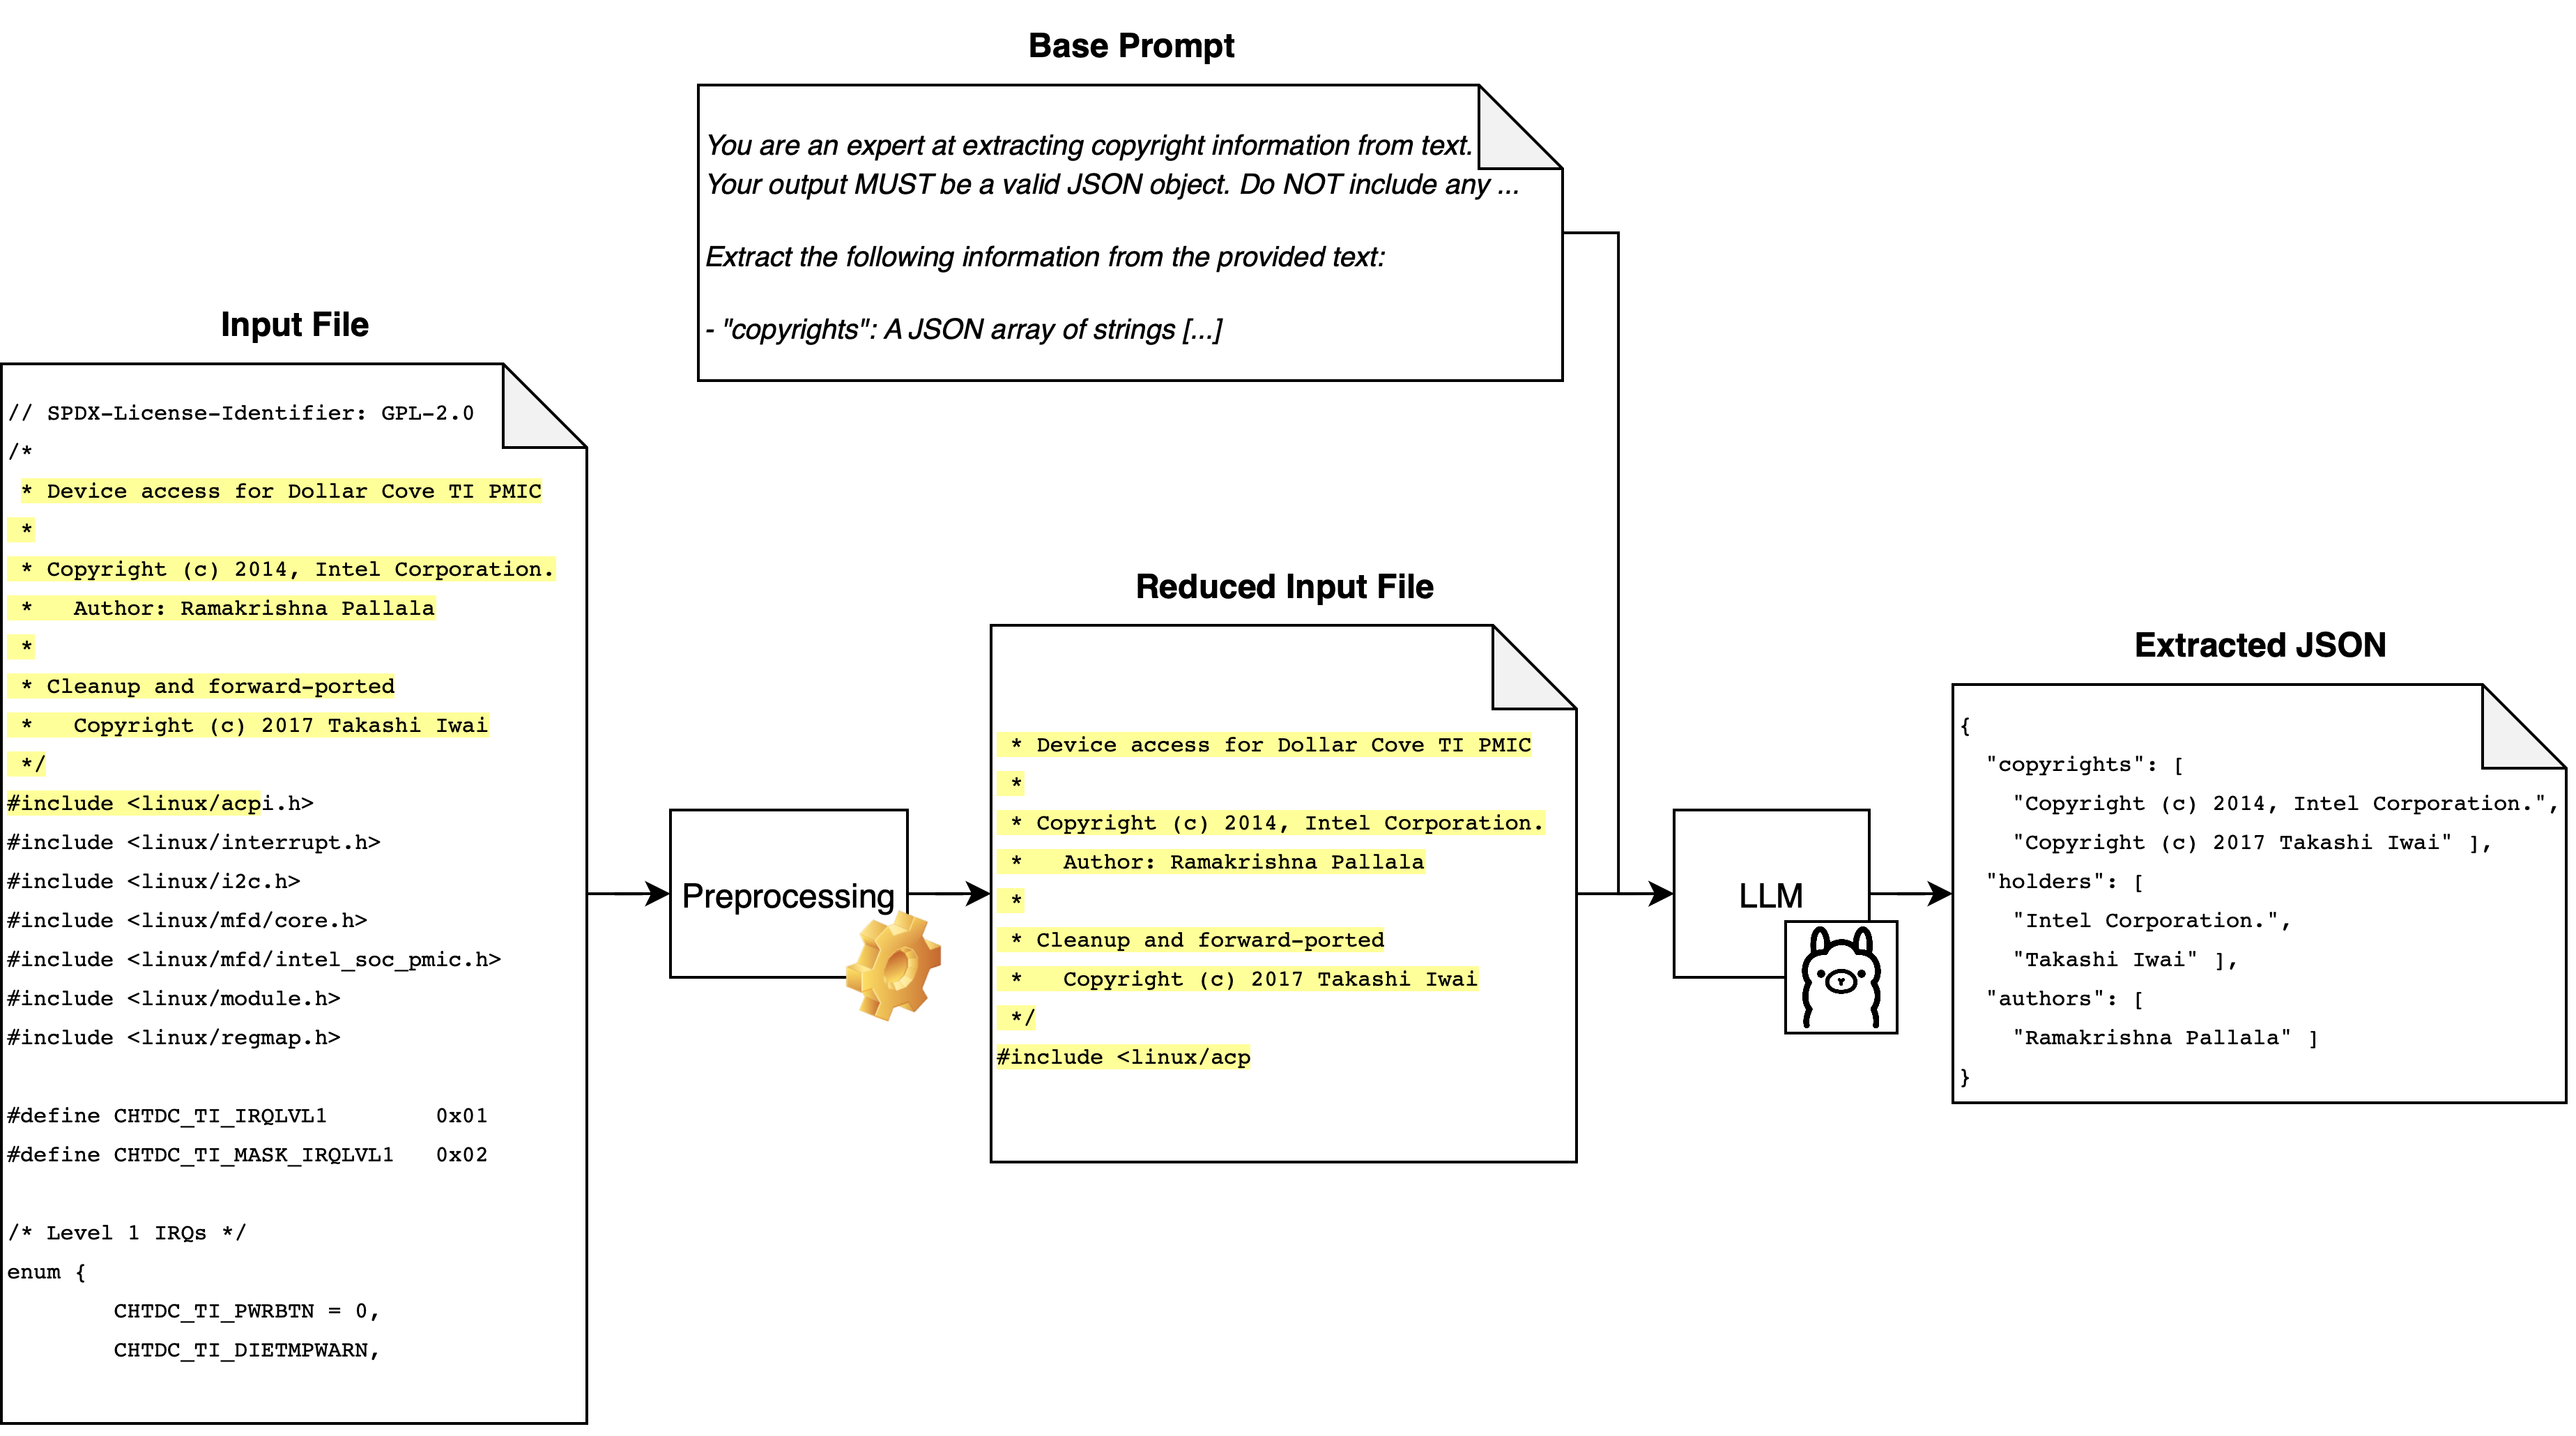
\includegraphics[width=1.3\textwidth]{benchmark/prompting}}
    \caption{Schematische Darstellung des Ablaufs der Inferenz. Zunächst wird die Eingabedatei mithilfe des Preprocessings auf relevante Inhalte reduziert und anschließend zusammen mit dem Eingabeprompt an das über Ollama ausgeführte LLM gesendet. Schließlich Antwortet das LLM mit den extrahierten Copyright-Informationen in einem strukturierten Format.}
    \label{fig:prompting_setup}
\end{figure}

% ----------------------------------------------------------------------------------------------------------------------

\subsection{Eingabeprompt}\label{subsec:eingabeprompt}

Der im Benchmark verwendete Eingabeprompt wurde mit dem Ziel entwickelt, die Modelle eindeutig und zuverlässig zur Extraktion von urheberrechtsrelevanten Informationen aus Texten anzuleiten.
Seine Struktur, sein Inhalt und seine Formatierung sind das Ergebnis iterativer Untersuchungen im Rahmen des \textit{Prompt-Engineering}, die in Kapitel~\ref{ch:prompt-engineering} detaillierter beschrieben werden.

Der Prompt beginnt mit einer expliziten Rollenzuweisung, indem das \gls{llm} als Experte für die Extraktion von Copyright-Informationen adressiert wird.
Anschließend folgt eine klare Anweisung, dass die Ausgabe ausschließlich in Form eines gültigen \gls{json}-Objekts erfolgen darf, ohne begleitende Erklärungen oder zusätzliche Inhalte.
Diese strikte Formatvorgabe dient der Sicherstellung konsistenter und maschinenlesbarer Ergebnisse, die unmittelbar in nachgelagerten Prozessen weiterverarbeitet werden können.

\begin{lstlisting}[keepspaces=true]
You are an expert at extracting copyright information from text.
Your output MUST be a valid JSON object. Do NOT include any additional text, comments, or explanations outside the JSON.
\end{lstlisting}

Inhaltlich ist der Prompt so gestaltet, dass er drei klar abgegrenzte Zielkategorien definiert: \textit{copyrights}, \textit{holders} und \textit{authors}.
Für jede Kategorie wird präzisiert, welche Informationen aus dem Eingabetext zu extrahieren sind und in welcher Form diese in das \gls{json}-Schema einzutragen sind.
Dabei werden auch Grenzfälle berücksichtigt, etwa die Behandlung von \enquote{All Rights Reserved}-Vermerken oder die explizite Auslassung Lizenzinformationen.

\begin{lstlisting}[keepspaces=true]
Extract the following information from the provided text into a JSON object with these keys:
- "copyrights": A JSON array of strings. Each string must be an EXACT, verbatim copythe actual copyright text. [...]
- "holders": A JSON array of strings. Each string must be the name of a copyright holder. [...]
- "authors": A JSON array of strings. Each string must be the name of an author mentioned in the context of copyright or authorship. [...]
\end{lstlisting}

Ein weiterer wichtiger Bestandteil des Prompts ist die Bereitstellung von Few-Shot-Beispielen, die sowohl Eingabetexte als auch die exakte Form der erwarteten Ausgabe zeigen.
Durch diese Demonstrationen wird das Modell mithilfe des \gls{icl} stärker in Richtung der gewünschten Struktur konditioniert und die Wahrscheinlichkeit von Abweichungen reduziert.

\begin{lstlisting}[keepspaces=true]
Example 1:
Text:
/*
Copyright (c) 2020 NVIDIA CORPORATION. All rights reserved.
Permission is hereby granted...
*/

Output:
{
  "copyrights": [ "Copyright (c) 2020 NVIDIA CORPORATION. All rights reserved." ],
  "holders": [ "NVIDIA CORPORATION" ],
  "authors": []
}
\end{lstlisting}

Am Ende des Prompts befindet sich ein Platzhalter, der während des Benchmarks durch den zu analysierenden Text ersetzt wird.
Damit bleibt der eigentliche Eingabeprompt inhaltlich konstant, während nur der relevante Dateiauszug dynamisch eingefügt wird.

\begin{lstlisting}[keepspaces=true]
Text to process:
{{FILE_CONTENT}}
\end{lstlisting}

% ----------------------------------------------------------------------------------------------------------------------

\subsection{Initiale und finale Durchführung}



% ======================================================================================================================

\section{Ergebnisse}\label{sec:ergebnisse-benchmark}

% Ergebnisse Exact Matches
% Ergebnisse F1-Score
% Ergebnisse pro Kategorie
% Ergebnisse Timeouts
% Ergebnisse Invalid-JSONs --> restored JSONs

% ======================================================================================================================

\section{Wahl des Modells}\label{sec:auswahl-modell-benchmark}
